% !TeX program = pdflatex
% Part VI of the godsil-gutman-lean series.
% The Walks That Remember the Cycles — a machine-checked sharp gap law between the
% matching polynomial and the non-backtracking spectrum in Lean 4.
% Build: pdflatex gap-window-lean.tex  (twice, for refs)
% Verified against the Lean source 2026-06-12 (lake build Ihara, 3054 jobs, exit 0;
% #print axioms SimpleGraph.treeLikeGap_eq_trace_hashimoto ->
% propext, Classical.choice, Quot.sound only). Toolchain v4.30.0-rc2, local Mathlib.

\documentclass[11pt]{article}
\usepackage[T1]{fontenc}
\usepackage{lmodern}
\usepackage{amsmath,amssymb,amsthm,booktabs,graphicx,hyperref}
\usepackage{xurl}
\usepackage[table]{xcolor}
\definecolor{ggteal}{HTML}{1B6F8C}
\definecolor{ggband}{HTML}{DCE7EB}
\definecolor{ggamber}{HTML}{E08A1E}
\usepackage[margin=1in]{geometry}
\usepackage{microtype}
\usepackage[most]{tcolorbox}
\usepackage{tikz}
\usetikzlibrary{arrows.meta,positioning}
\setlength{\emergencystretch}{4em}
\graphicspath{{figures/}}
\newtheorem{theorem}{Theorem}
\newtheorem{lemma}{Lemma}
\newtheorem{definition}{Definition}
\newcommand{\lean}[1]{\texttt{#1}}
\newcommand{\Z}{\mathbb{Z}}
\newcommand{\R}{\mathbb{R}}
\newcommand{\N}{\mathbb{N}}
\newcommand{\C}{\mathbb{C}}
\DeclareMathOperator{\tr}{tr}
\hypersetup{colorlinks=true,linkcolor=ggteal,citecolor=ggteal,urlcolor=ggteal}
\newtcbox{\keybox}{on line,boxrule=0.9pt,colframe=ggteal,colback=ggband!40,
  arc=3pt,left=8pt,right=8pt,top=5pt,bottom=5pt}
\newcommand{\keyeq}[1]{\begin{center}\keybox{$\displaystyle #1$}\end{center}}

\title{\bf The Walks That Remember the Cycles\\[4pt]
  \large\normalfont A machine-checked sharp gap law between the matching polynomial\\
  and the non-backtracking spectrum in Lean~4}
\author{Carles Mar\'in\thanks{Formalized with AI assistance (Claude, Anthropic); the mathematics
and all claims are the author's responsibility. The methodology is discussed in
Section~\ref{sec:boundary}.}\\[3pt]
  \normalsize Independent researcher\\
  \normalsize \texttt{karlesmarin@gmail.com}}
\date{June 2026}

\begin{document}
\maketitle

\begin{abstract}
I present a machine-checked, \lean{sorry}-free proof, in Lean~4 over Mathlib, of the
\emph{sharp trace-formula gap law} for a finite simple graph of girth $g$: for every
$1 \le k \le g+1$,
\[
\tr A^k \;-\; p_k \;=\; \tr B^k,
\]
where $A$ is the adjacency matrix, $B$ the Hashimoto non-backtracking operator, and
$p_k = \sum_i \theta_i^k$ the power sums of the roots of the matching polynomial. Below the
girth both sides vanish; at $k \in \{g, g+1\}$ both sides count the rooted traversals of the
$k$-cycles, $2k\,c_k$; and the window is sharp---the law fails at $k = g+2$ on every
graph we tested, including all $12\,064$ connected cyclic graphs on $4$ to $8$ vertices.
The proof is assembled from pieces of independent use: a cycle-extraction lemma for
non-backtracking chains; a parity lemma for edge incidences of \emph{arbitrary} closed walks
(Mathlib's version carries a trail hypothesis its own proof does not use); an exact
incidence count for cycles; and a structure theorem---in the window, the closed
non-backtracking walks, the rooted cycle traversals, and the closed walks that fail to lift
to Godsil's path tree are the \emph{same} family, counted three ways. The headline theorem
depends only on the three standard axioms. I am exact about the boundary: the mathematics is
classical (Ihara, Hashimoto, Bass, Godsil; the law itself is folklore-adjacent and known to
coding theorists in other clothing); the contribution is the formalization---to the best of
my knowledge the first machine-checked bridge between the matching polynomial and the
non-backtracking spectrum in any proof assistant---and the sharp window is stated and proved
as such. A companion paper applies the law, as a certified census of short cycles, to the
LDPC codes deployed in the IEEE 802.11n (WiFi) standard.
\end{abstract}

\noindent\emph{Reader's map.} If you read only one thing, read Theorem~\ref{thm:gaplaw} and
Figure~\ref{fig:window}---the statement, and the picture of the law holding on its window and
breaking, spectacularly, just past it. The proof is a single chain (Figure~\ref{fig:readermap});
every link has its own section and its own Lean name (Table~\ref{tab:results}). The honest
limits are in Section~\ref{sec:boundary}.

\begin{figure}[h]
\centering
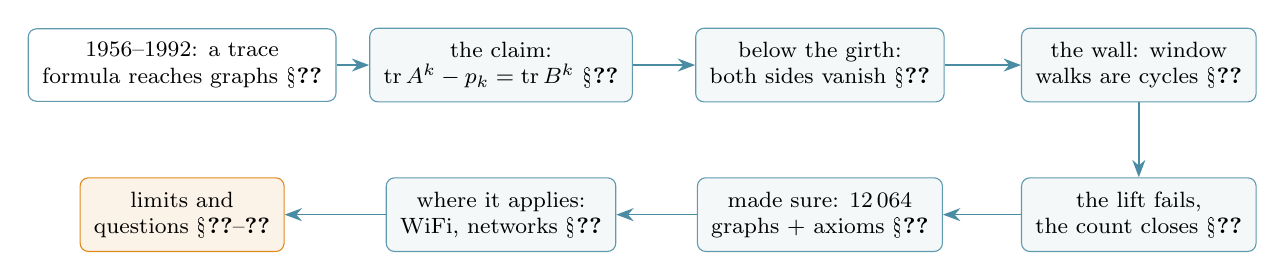
\begin{tikzpicture}[
  theme/.style={draw=ggteal!70,fill=ggband!30,rounded corners=3pt,align=center,
    inner sep=5pt,font=\footnotesize,minimum height=9mm},
  hist/.style={draw=ggteal!70,fill=white,rounded corners=3pt,align=center,
    inner sep=5pt,font=\footnotesize,minimum height=9mm},
  last/.style={draw=ggamber,fill=ggamber!10,rounded corners=3pt,align=center,
    inner sep=5pt,font=\footnotesize,minimum height=9mm},
  flow/.style={-{Stealth[length=2.2mm]},semithick,ggteal!80}]
  \node[hist]  (a) at (0,1.5)    {1956--1992: a trace\\formula reaches graphs\ \S\ref{sec:intro}};
  \node[theme] (b) at (4.05,1.5) {the claim:\\$\tr A^k - p_k = \tr B^k$\ \S\ref{sec:claim}};
  \node[theme] (c) at (8.1,1.5)  {below the girth:\\both sides vanish\ \S\ref{sec:stoneA}};
  \node[theme] (d) at (12.15,1.5){the wall: window\\walks are cycles\ \S\ref{sec:wall}};
  \node[theme] (e) at (12.15,-0.4){the lift fails,\\the count closes\ \S\ref{sec:count}};
  \node[theme] (f) at (8.1,-0.4) {made sure: $12\,064$\\graphs + axioms\ \S\ref{sec:verification}};
  \node[theme] (g) at (4.05,-0.4){where it applies:\\WiFi, networks\ \S\ref{sec:applications}};
  \node[last]  (h) at (0,-0.4)   {limits and\\questions\ \S\ref{sec:boundary}--\ref{sec:questions}};
  \draw[flow] (a) -- (b);
  \draw[flow] (b) -- (c);
  \draw[flow] (c) -- (d);
  \draw[flow] (d) -- (e);
  \draw[flow] (e) -- (f);
  \draw[flow] (f) -- (g);
  \draw[flow] (g) -- (h);
\end{tikzpicture}
\caption{The reader's map: the claim, the three stones of its proof, the checks, the uses,
and what remains.}
\label{fig:readermap}
\end{figure}

% ---------------------------------------------------------------
\section{Introduction: a trace formula comes down a ladder}
\label{sec:intro}

Why should two censuses with no shared definition ever agree? Begin with the anomaly. Take
the Petersen graph and run two censuses that have no obvious business agreeing: count all closed walks of length $k$ and subtract those that lift to
Godsil's path tree ($\tr A^k - p_k$); separately, count the closed walks that never
immediately backtrack ($\tr B^k$). At $k = 5$ both give $120$. At $k = 6$, both give $120$
again. At $k = 7$ the first census jumps to $1680$---and the second collapses to $0$,
because the Petersen graph has no $7$-cycles at all (Figure~\ref{fig:window}). Two censuses
in lockstep, then a cliff. The lockstep is a theorem; the cliff is its sharpness; this paper
machine-checks both. Where does such a pair of censuses come from?

In 1956 Selberg proved a formula that holds two ways of hearing a hyperbolic surface against
each other: on one side the spectrum of the Laplacian, on the other the lengths of the closed
geodesics~\cite{Selberg1956}. Ten years later Ihara, working $p$-adically, found the discrete
shadow of that formula: a zeta function for a graph, built from its closed geodesics---the
closed walks that never immediately backtrack~\cite{Ihara1966}. What had been analysis on a
surface became linear algebra on a finite object: Hashimoto encoded the non-backtracking
condition as a $0/1$ matrix $B$ on directed edges~\cite{Hashimoto1989}, and Bass proved that
its characteristic polynomial factors through the adjacency matrix~\cite{Bass1992}---the
graph-theoretic Selberg identity, formalized in the Ihara--Bass companion of this
series~\cite{MarinBass2026}.

A trace formula needs a second side. On a surface it is the Plancherel term, the contribution
of the universal cover; on a graph the universal cover is a tree, and the object that hears
the tree is the \emph{matching polynomial}: Godsil proved in 1981 that the power sums of its
roots count the closed walks that lift to the \emph{path tree}---the ``tree-like''
walks~\cite{Godsil1981}, a theorem this series formalized in Part~IV~\cite{MarinMoment2026},
building on the path-tree bijection of Part~III~\cite{MarinPTW2026} and resting on the
real-rootedness of Heilmann and Lieb~\cite{HeilmannLieb1972} formalized in
Part~II~\cite{MarinHL2026}.

So by Part~V the series had built, separately, the two sides of a trace formula: the
tree side ($p_k$, matching polynomial, path tree) and the geodesic side ($\tr B^k$,
non-backtracking operator, Ihara zeta). Each had its own paper, its own verifier runs, its own
Zenodo record. They had never met inside the proof assistant.

This paper is the meeting. The bridge is a subtraction:
\[
\tr A^k \;-\; p_k,
\]
all closed walks minus the tree-like ones---the walks the tree cannot explain. The theorem is
that on a sharp window, $1 \le k \le g+1$ with $g$ the girth, this remainder \emph{is} the
non-backtracking trace $\tr B^k$: what walks forget about the tree, they remember about the
cycles. The window is exact. One step past it, at $k = g+2$, the first walk appears that
wraps a cycle and then wanders---and the two sides come apart, on every graph we tested
(Figure~\ref{fig:window}). The payoff of the necklace is that this is the first theorem of
the series that \emph{consumes both strands at once}: its Lean proof imports the path-tree
and moment machinery of Parts~III--IV and the Hashimoto operator of the Ihara--Bass companion
in the same file, and neither side could be stated without the other's vocabulary.

% ---------------------------------------------------------------
\section{The claim: the law and its terms}
\label{sec:claim}

What, exactly, is being subtracted on the left side of the law? Throughout, $G$ is a finite
simple graph on vertex set $V$, $A$ its adjacency matrix, and $g$ its girth (the length of a shortest cycle; $g \ge 3$). The matching polynomial is
\[
\mu_G(x) \;=\; \sum_{j \ge 0} (-1)^j\, m_j\, x^{\,n-2j},
\]
with $m_j$ the number of $j$-edge matchings, and $p_k = \sum_{i} \theta_i^k$ the $k$-th power
sum of its roots (over $\C$; the roots are in fact real~\cite{HeilmannLieb1972,MarinHL2026}).
The Hashimoto operator $B$ acts on the $2|E|$ \emph{darts} (ordered edges): $B_{d,e} = 1$
exactly when $e$ continues $d$ without reversing it ($\mathrm{snd}\,d = \mathrm{fst}\,e$ and
$e \neq \bar d$)~\cite{Hashimoto1989,MarinBass2026}.

\begin{theorem}[the sharp gap law; \lean{trace\_sub\_matchingPowerSum\_eq\_trace\_hashimoto}]
\label{thm:gaplaw}
For every $k$ with $1 \le k \le g+1$,
\keyeq{\tr A^k \;-\; p_k \;=\; \tr B^k .}
Below the girth ($k < g$) both sides are $0$. At $k \in \{g, g+1\}$ both sides equal
$2k\,c_k$, where $c_k$ is the number of $k$-cycles of $G$.
\end{theorem}

The Lean statement is exactly this, over $\C$, with $p_k$ the literal
\lean{Multiset.sum} of $k$-th powers of the roots of \lean{matchingPoly} mapped into $\C$;
the integer form \lean{treeLikeGap\_eq\_trace\_hashimoto} states the same identity over $\Z$
with $p_k$ replaced by Godsil's tree-like walk count, and the two are joined by Part~IV's
moment theorem. No regularity, connectivity or bipartiteness is assumed. The artifact
itself, verbatim:
\begin{tcolorbox}[colframe=ggteal!70,colback=ggband!20,arc=3pt,boxrule=0.8pt]
\small\begin{verbatim}
theorem trace_sub_matchingPowerSum_eq_trace_hashimoto
    [Fintype V] [DecidableEq V] [DecidableRel G.Adj]
    {k : N} (hk : 0 < k) (hwin : (k : N_inf) <= G.egirth + 1) :
    ((G.adjMatrix N ^ k).trace : C) - G.matchingPowerSum k
      = ((G.hashimoto C) ^ k).trace
\end{verbatim}
\end{tcolorbox}

One example fits in the head. On the triangle $K_3$ at $k = g = 3$: there are six closed
walks of length $3$ (three base points, two directions), so $\tr A^3 = 6$; none of them is
tree-like---a walk around a triangle does not lift to a tree---and indeed $p_3 = 0$, since
$\mu_{K_3} = x^3 - 3x$ has roots $0, \pm\sqrt3$ whose cubes cancel; and every one of the six
is non-backtracking, so $\tr B^3 = 6$. The law reads $6 - 0 = 6$, and each number is
checkable without paper. The theorem is that this never fails until $k = g+2$.

Three remarks before the proof. First, the subtraction is meaningful because of Part~IV:
$p_k$ \emph{is} a count of walks (the tree-like ones), so the left side is a difference of
two censuses of the same population. Second, the right side is also a census: $\tr B^k$
counts the closed non-backtracking dart walks of length $k$
(\lean{trace\_hashimoto\_pow}, mapped in the Jacobi--Newton companion~\cite{MarinJN2026}). The theorem is therefore a \emph{bijection of censuses}, and that
is how it is proved. Third, the window matters: for $k \ge g+2$ the law is not merely
unproved but \emph{false}, and visibly so (Figure~\ref{fig:window};
Section~\ref{sec:verification})---a single exact counterexample (Petersen at $k = 7$, where
$\tr A^7 - p_7 = 1680$ while $\tr B^7 = 0$) shows the window cannot be widened. That the
failure is \emph{universal} beyond $g+2$ is tested across $12\,064$ graphs, not formalized:
the theorem is the window equality, and ``sharp'' means the window cannot be extended.

\begin{figure}[t]
\centering
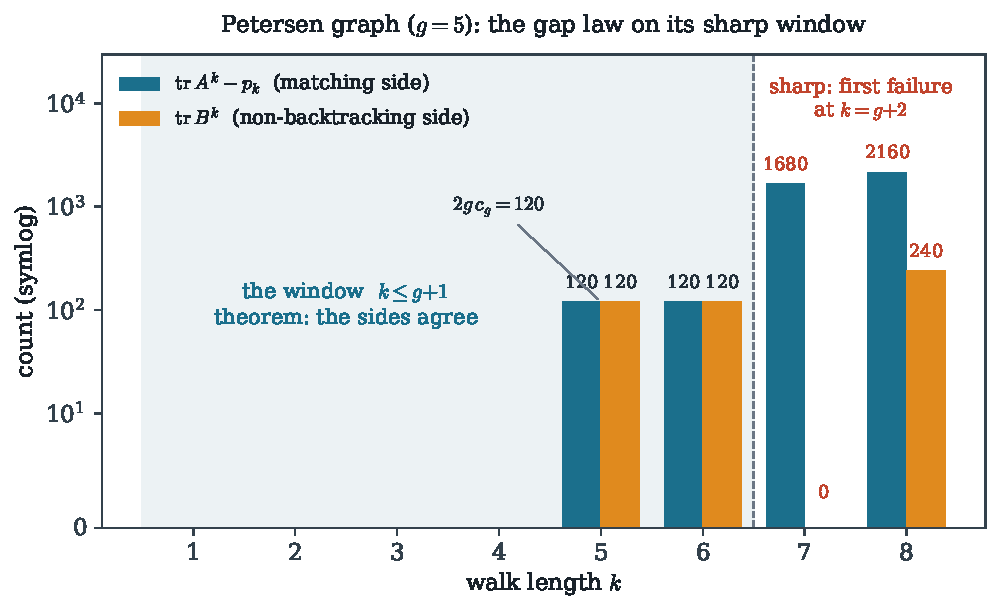
\includegraphics[width=0.92\textwidth]{gw_fig1_window}
\caption{The gap law on the Petersen graph ($g = 5$), in exact integer arithmetic. On the
window $k \le 6$ the two censuses agree---both are $0$ below the girth and $120 = 2\cdot 5
\cdot 12$ at $k = 5$ (Petersen has twelve pentagons), $120 = 2 \cdot 6 \cdot 10$ at $k = 6$
(ten hexagons). At $k = 7$ the law breaks as violently as it can: the left side jumps to
$1680$ while the right side is $0$---the Petersen graph famously has no $7$-cycles, so there
are no closed non-backtracking walks of length $7$ at all, while $1680$ closed walks of
length $7$ already fail to be tree-like (a pentagon plus a dangling edge). Sharpness is not
an artifact of one graph: it holds on all $12\,064$ connected cyclic graphs on $4$ to $8$
vertices (Section~\ref{sec:verification}).}
\label{fig:window}
\end{figure}

\begin{table}[h]
\centering\small
\rowcolors{2}{ggband!35}{white}
\begin{tabular}{@{}rrrrr@{}}
\toprule
\rowcolor{ggteal!18} $k$ & $\tr A^k$ & $p_k$ & $\tr A^k - p_k$ & $\tr B^k$ \\
\midrule
1 & 0    & 0    & 0    & 0   \\
2 & 30   & 30   & 0    & 0   \\
3 & 0    & 0    & 0    & 0   \\
4 & 150  & 150  & 0    & 0   \\
5 & 120  & 0    & \textbf{120}  & \textbf{120} \\
6 & 990  & 870  & \textbf{120}  & \textbf{120} \\
7 & 1680 & 0    & {\color{ggamber}1680} & {\color{ggamber}0}   \\
8 & 7590 & 5430 & {\color{ggamber}2160} & {\color{ggamber}240} \\
\bottomrule
\end{tabular}
\caption{The Petersen data behind Figure~\ref{fig:window}: spectra give
$\tr A^k = 3^k + 5 + 4(-2)^k$; $p_k$ by Newton's identities from
$\mu = x^{10} - 15x^8 + 75x^6 - 145x^4 + 90x^2 - 6$; $\tr B^k$ by the Ihara--Bass
per-eigenvalue recurrence $s_k = \lambda s_{k-1} - 2 s_{k-2}$ plus $5(1 + (-1)^k)$. The
window (bold) and the first two failures (amber). Every entry is exact.}
\label{tab:petersen}
\end{table}

% ---------------------------------------------------------------
\section{Stone A: nothing below the girth}
\label{sec:stoneA}

Below the girth the law reads $0 = 0$---so why is neither zero free? Serre's \emph{Trees}
taught a generation the slogan: below its girth, a graph cannot tell itself apart from its
universal cover~\cite{Serre1980}. A formal proof cannot wave at a
cover; it needs the slogan as a finite witness.

Take the right side first: why is there no closed non-backtracking walk shorter than the
shortest cycle? Classically one waves
at the universal cover; the formal proof wants a finite witness, and the witness is a
\emph{cycle extracted from the walk itself}.

\begin{lemma}[cycle extraction; \lean{Walk.exists\_isCycle\_of\_nbChain\_of\_not\_nodup}]
\label{lem:crux}
Let $w$ be a walk whose darts form a non-backtracking chain and whose vertex support repeats
a vertex. Then $G$ contains a cycle of length at most the length of $w$, supported on the
edges of $w$.
\end{lemma}

The proof is a structural induction with no rotation anywhere---rotating a walk would break
the \emph{linear} non-backtracking chain at the seam, an obstruction that silently corrupts
informal proofs. If the tail of the walk already repeats a vertex, induct. Otherwise the
head vertex $u$ re-enters the tail; the prefix up to that re-entry is a path
(\lean{IsPath.takeUntil}), and the closing edge either avoids the path---then
\lean{cons\_isCycle\_iff} hands us the cycle---or lies on it, which pins the path to the
single reversed dart of the entering edge and contradicts the chain at its first link.
Stone~A follows by a pigeonhole: a closed non-backtracking dart walk of length $k$ presents
$k+1$ darts whose last repeats its first, hence at most $k$ distinct edges; the extracted
cycle needs at least $g$ of them; so $k \ge g$
(\lean{relWalks\_nbRel\_closed\_eq\_empty}, \lean{trace\_hashimoto\_pow\_eq\_zero\_of\_lt\_egirth}).
The left side's $0$ is Part~III's below-girth theorem (every short closed walk lifts to the
path tree). The gap law below the girth is then a subtraction of zeros---but each zero is a
theorem.

% ---------------------------------------------------------------
\section{The wall: window walks are cycles}
\label{sec:wall}

Why is a closed non-backtracking walk in the window forced to be a cycle? The oldest blade
in the book is Euler's, K\"onigsberg, 1736: every entrance needs an exit~\cite{Euler1736}. Three centuries later the same parity argument decides the case that
modern hypotheses cannot reach.

The content of the law lives at $k \in \{g, g+1\}$, and it is a \emph{structure} theorem:

\begin{theorem}[window rigidity; \lean{Walk.isCycle\_of\_nbChain\_window}]
\label{thm:rigidity}
A closed non-backtracking walk of length $k$ with $1 \le k \le g+1$ is a cycle.
\end{theorem}

What surprised us in the formalization is how little ``non-backtracking'' the proof
ultimately uses: the chain hypothesis enters \emph{only} through Lemma~\ref{lem:crux}. The
extracted cycle $C$ satisfies $g \le |C| \le k \le g+1$, leaving exactly two cases, and both
die by counting edge incidences---parity and degree, nothing else.

\emph{The parity blade.} For any walk, count the edge slots incident to a vertex $x$.
Mathlib proves the parity of this count for \emph{trails}
(\lean{IsTrail.even\_countP\_edges\_iff}), but its own induction never uses the trail
hypothesis except to feed itself; removing it
(\lean{Walk.even\_countP\_edges\_iff'}) gives: in a \emph{closed} walk, every vertex has
even incidence count. This matters because the walks in case $|C| = k-1$ need not be trails.

\emph{The degree blade.} A cycle meets each vertex of its support in exactly two edge slots
(\lean{Walk.countP\_edges\_of\_isCycle}), a transfer of Mathlib's
\lean{ncard\_neighborSet\_toSubgraph\_eq\_two} along an explicit two-sided bijection
$e \mapsto$ ``the other endpoint''.

\emph{Case $|C| = k-1$.} The walk's edge multiset is the cycle's edges plus one extra slot
$f$ (a multiset surgery isolates $f$). Any endpoint $x$ of $f$ then has incidence
$2 + 1 = 3$ or $0 + 1 = 1$---odd either way, against the parity blade. No such walk exists
(\lean{Walk.not\_closed\_of\_isCycle\_edges\_add\_one}).

\emph{Case $|C| = k$.} The walk's edges are a permutation of the cycle's, so the walk is a
trail. If its support repeated an interior vertex $x$, rotate the walk to base $x$
(legitimate here---trails survive rotation, and we no longer need the chain): $x$ now sits
at three pairwise-distinct slots $\{0, m-1, m\}$, giving three \emph{distinct} edges at $x$,
against the degree blade's two. So the support is simple and the walk is the cycle
(\lean{Walk.isCycle\_of\_edges\_perm}).

Composing the two cases with Lemma~\ref{lem:crux} proves Theorem~\ref{thm:rigidity}. The
window hypothesis is used exactly once---to squeeze $|C|$ into $\{k-1, k\}$---and this is
precisely what fails at $k = g+2$: a $g$-cycle plus a $2$-step excursion becomes available,
parity is satisfied ($2+2$), and the law breaks
(Figures~\ref{fig:window} and~\ref{fig:families}).

\begin{figure}[t]
\centering
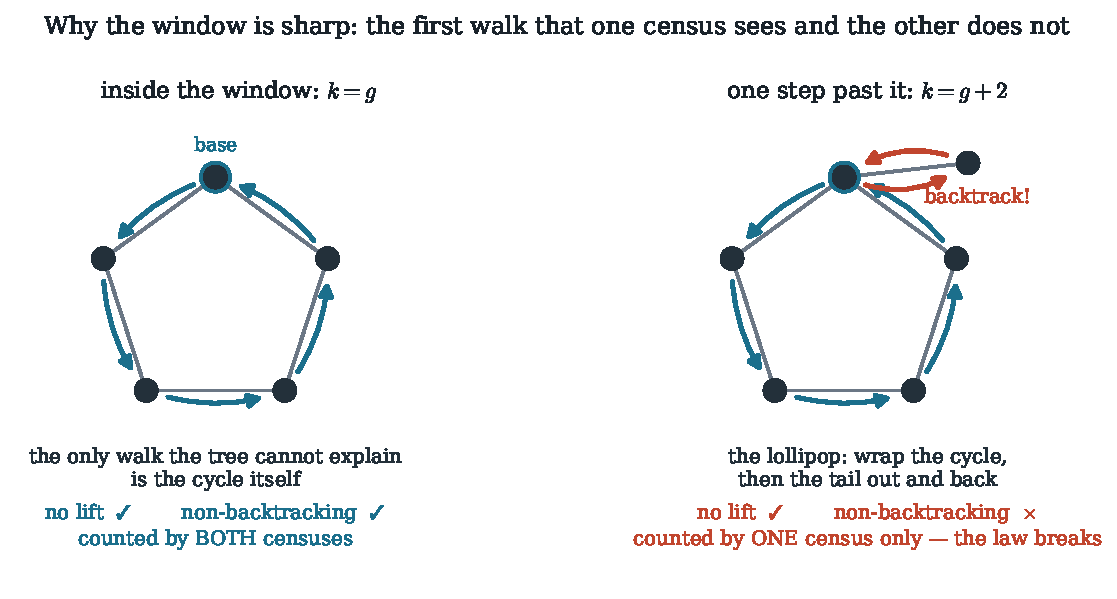
\includegraphics[width=0.92\textwidth]{gw_fig2_families}
\caption{The structure theorem in one picture. Left: inside the window the only closed walk
the path tree cannot explain is a cycle traversal, and a cycle never backtracks---the two
censuses count the same object. Right: at $k = g+2$ the first \emph{lollipop} appears: it
wraps the pentagon (so it does not lift; the matching census counts it) but its tail turns
back on itself (so the non-backtracking census rejects it). One walk, one census,
no law.}
\label{fig:families}
\end{figure}

% ---------------------------------------------------------------
\section{The other side, and the count that closes the bridge}
\label{sec:count}

When does a closed walk refuse to lift to the path tree---and why is that the very thing
that makes it a cycle? Counting by bijection is combinatorics' oldest trust protocol:
Pr\"ufer certified Cayley's $n^{n-2}$ by exhibiting the correspondence, one tree at a
time~\cite{Prufer1918}. The gap
law closes the same way, one walk at a time.

The left census needs the mirror statement: in the window, a closed walk fails to lift to the
path tree \emph{exactly when} it is a cycle. One direction is a pleasant computation in the
lift itself: along a cycle the stack only ever extends, and at the closing step the root is
in the stack but is not its penultimate entry, so the retreat fails
(\lean{Walk.not\_isTreeLike\_of\_isCycle}). The other direction needed, on paper, a second
wall---and dissolved instead into pieces already proved: if a window walk does not lift,
its edge support contains a cycle (the contrapositive of Part~III's
\lean{isTreeLike\_of\_acyclic}); mapping that cycle into $G$ lands exactly in the two cases
of Section~\ref{sec:wall}, whose conclusions now read ``the walk is that cycle'' or
``false'' (\lean{Walk.isCycle\_or\_isTreeLike\_window}).

So in the window three families coincide:
\keyeq{\{\text{closed NB dart walks}\} \;=\; \{\text{rooted cycle traversals}\} \;=\;
\{\text{closed walks that do not lift}\},}
and the gap law is the statement that the first and third have the same cardinality. The
final bijection (\lean{sum\_card\_not\_treeLike\_eq\_sum\_card\_relWalks}) sends a
non-lifting walk---now known to be a cycle---to its dart list closed by the repeat of its
first dart; injectivity rests on a small lemma of independent value, \emph{a walk is
determined by its darts} (\lean{Walk.eq\_of\_darts\_eq}); surjectivity reassembles the walk
from the dart list with Mathlib's \lean{Walk.ofDarts}. Summing over roots and casting
through $\Z$ gives the capstone, and Part~IV's moment theorem rewrites the tree-like count
as $p_k$: Theorem~\ref{thm:gaplaw}.

\begin{table}[t]
\centering\small
\rowcolors{2}{ggband!35}{white}
\begin{tabular}{@{}lll@{}}
\toprule
\rowcolor{ggteal!18} Lean name & statement & where \\
\midrule
\lean{trace\_sub\_matchingPowerSum\_eq\_trace\_hashimoto} & $\tr A^k - p_k = \tr B^k$ on the window & \S\ref{sec:claim} \\
\lean{treeLikeGap\_eq\_trace\_hashimoto} & the capstone over $\Z$ & \S\ref{sec:claim} \\
\lean{exists\_isCycle\_of\_nbChain\_of\_not\_nodup} & cycle extraction from an NB chain & \S\ref{sec:stoneA} \\
\lean{trace\_hashimoto\_pow\_eq\_zero\_of\_lt\_egirth} & $\tr B^k = 0$ for $k < g$ & \S\ref{sec:stoneA} \\
\lean{even\_countP\_edges\_iff'} & incidence parity, no trail hypothesis & \S\ref{sec:wall} \\
\lean{countP\_edges\_of\_isCycle} & a cycle has incidence count $2$ & \S\ref{sec:wall} \\
\lean{not\_closed\_of\_isCycle\_edges\_add\_one} & no walk is a cycle plus one slot & \S\ref{sec:wall} \\
\lean{isCycle\_of\_edges\_perm} & a closed walk on a cycle's edges is the cycle & \S\ref{sec:wall} \\
\lean{isCycle\_of\_nbChain\_window} & window rigidity (Theorem~\ref{thm:rigidity}) & \S\ref{sec:wall} \\
\lean{not\_isTreeLike\_of\_isCycle} & a cycle does not lift to the path tree & \S\ref{sec:count} \\
\lean{isCycle\_or\_isTreeLike\_window} & the window dichotomy & \S\ref{sec:count} \\
\lean{eq\_of\_darts\_eq} & a walk is determined by its darts & \S\ref{sec:count} \\
\lean{sum\_card\_not\_treeLike\_eq\_sum\_card\_relWalks} & the bijection of censuses & \S\ref{sec:count} \\
\bottomrule
\end{tabular}
\caption{The load-bearing results, all \lean{sorry}-free in
\lean{Ihara/NbVanishing.lean} and \lean{Ihara/GapWindow.lean} of the repository. Axioms of
the capstone: \lean{propext}, \lean{Classical.choice}, \lean{Quot.sound} only.}
\label{tab:results}
\end{table}

% ---------------------------------------------------------------
\section{Made sure: twelve thousand graphs and three axioms}
\label{sec:verification}

If a formal proof is already certain, what work is left for twelve thousand graphs?
Numerical evidence is a compass, not a deed: Mertens' conjecture agreed with every computer
ever pointed at it and fell anyway~\cite{OdlyzkoTeRiele1985}. The two instruments here divide
the labor in the opposite direction---the numerics choose the statement, the proof assistant
owns it.

Formal proofs eliminate one kind of error; choosing the \emph{right statement} requires
another instrument, and the statement here---in particular the claim that the window is
sharp---was locked numerically before a line of Lean was written, and re-locked after.

\begin{table}[h]
\centering\small
\rowcolors{2}{ggband!35}{white}
\begin{tabular}{@{}lrrrrr@{}}
\toprule
\rowcolor{ggteal!18} graph & $g$ & $c_g$ & $\mathrm{gap}_g = \tr B^g$ & window verified & first failure \\
\midrule
$K_3$        & 3 & 1  & 6   & $k \le 4$ & $k=5$ \\
$C_5$        & 5 & 1  & 10  & $k \le 6$ & $k=7$ \\
$K_4$        & 3 & 4  & 24  & $k \le 4$ & $k=5$ \\
$K_{3,3}$    & 4 & 9  & 72  & $k \le 5$ & $k=6$ \\
$Q_3$ (cube) & 4 & 6  & 48  & $k \le 5$ & $k=6$ \\
Petersen     & 5 & 12 & 120 & $k \le 6$ & $k=7$ \\
\midrule
\multicolumn{6}{l}{\emph{exhaustive sweep}: all $12\,064$ connected cyclic graphs, $4 \le n \le 8$
(Sage, \lean{nauty\_geng}):} \\
\multicolumn{6}{l}{\quad $0$ violations on the window; the law failed at $k = g+2$ on
\emph{every single graph}.} \\
\bottomrule
\end{tabular}
\caption{Numerical locks. The named graphs are checked in exact arithmetic
(\lean{research/\_tmp/traceformula\_lock.py}); the sweep
(\lean{research/\_tmp/gaplaw\_sweep.py}) computes both sides independently---$B$ as an
explicit dart matrix, $p_k$ by Newton from matching counts---and confirms that sharpness at
$g+2$ is universal in this range, not generic.}
\label{tab:locks}
\end{table}

On the formal side: the development builds with Lean toolchain v4.30.0-rc2 against a pinned
Mathlib (3054 jobs, exit 0), the two new files are warning-free, and
\lean{\#print axioms} on every theorem of Table~\ref{tab:results} reports
\lean{propext}, \lean{Classical.choice}, \lean{Quot.sound}---the three standard axioms---and
nothing else. No \lean{native\_decide}, no \lean{Decide}-bombs, no custom axioms.

Checking this paper is three commands:
\begin{tcolorbox}[colframe=ggteal!70,colback=ggband!20,arc=3pt,boxrule=0.8pt]
\footnotesize\begin{verbatim}
git clone https://github.com/karlesmarin/godsil-gutman-lean
cd godsil-gutman-lean && lake exe cache get && lake build Ihara
echo 'import Ihara.GapWindow
      #print axioms
        SimpleGraph.trace_sub_matchingPowerSum_eq_trace_hashimoto' \
  | lake env lean --stdin
\end{verbatim}
\end{tcolorbox}

% ---------------------------------------------------------------
\section{Where it applies: from a trace identity to a WiFi chip}
\label{sec:applications}

What does a machine-checked trace identity buy an engineer that a faster algorithm does not?
Gallager invented LDPC codes in 1962 and the world shelved them for thirty
years~\cite{Gallager1962}; when they returned (to WiFi, to 5G, to deep space), the girth of
a graph had become an engineering quantity. That is where a trace identity meets a chip.

\emph{Certified cycle censuses.} At $k = g$ the law is a formula for the number of shortest
cycles, $c_g = (\tr A^g - p_g)/2g$, computable from the spectrum and the first few matching
counts. Short cycles in the Tanner graph of an LDPC code degrade belief-propagation
decoding, and counting them is an established engineering task~\cite{KarimiBanihashemi2013,
BlakeLin2018}. The companion paper applies the (now theorem-backed) formula as a
\emph{certified census} to the four LDPC codes of IEEE 802.11n at $n = 648$: three mutually
independent computations agree exactly on all four---$c_6 = 3942$ (rate $1/2$), $c_6 = 8046$
(rate $2/3$), $c_4 = 54$ (rate $3/4$, where the girth collapses to $4$), $c_6 = 32\,346$
(rate $5/6$). The certification layer, not the counting speed, is the contribution there:
the counting algorithms of~\cite{KarimiBanihashemi2013,BlakeLin2018} are faster and reach
further ($k \le 2g-2$), but carry no machine-checked guarantee.

\begin{tcolorbox}[colframe=ggamber,colback=ggamber!8,arc=3pt,boxrule=0.8pt,
  title=\textbf{The recipe: count your graph's shortest cycles in four lines},
  coltitle=white,colbacktitle=ggamber]
Given a graph with girth $g$ (even case shown; $m_j$ = number of $j$-matchings):
(1) compute $\tr A^g$ from the spectrum or by matrix powers;
(2) count the small matchings, $m_1 = |E|$, $m_2 = \binom{m_1}{2} - \sum_v \binom{d_v}{2}$,
\dots\ up to $m_{g/2}$;
(3) Newton: $p_2 = 2m_1$, $p_4 = 2m_1^2 - 4m_2$, $p_6 = 2m_1^3 - 6m_1m_2 + 6m_3$;
(4) then $c_g = (\tr A^g - p_g)/2g$, with a machine-checked guarantee.
\emph{Worked:} $K_{3,3}$ has $g = 4$, eigenvalues $\pm 3, 0^4$, so $\tr A^4 = 162$;
$m_1 = 9$, $m_2 = \binom92 - 6\binom32 = 18$, so $p_4 = 2\cdot 81 - 4\cdot 18 = 90$;
hence $c_4 = (162 - 90)/8 = 9$: the nine quadrilaterals of $K_{3,3}$, certified.
\end{tcolorbox}

\emph{Chemistry: the matching polynomial is measurable.} In the H\"uckel theory of
conjugated hydrocarbons, $\mu_G$ is the \emph{reference polynomial}: the topological
resonance energy of a molecule is the difference between the spectra of $A$ (the
$\pi$-system) and of $\mu_G$ (the same system with its cycles erased)---aromaticity as a
spectral gap between a graph and its own tree shadow~\cite{Aihara1976,Gutman1979}. The gap
law is the walk-level identity beneath that chemistry: it says \emph{exactly which} walk
counts the two spectra share (all of them, up to $g+1$) and where they first part. The
$k$-th moments of benzene's $\pi$-system and of its reference polynomial agree until $k = 6$
wraps the hexagon---which is the aromatic sextet seen combinatorially.

\emph{Epidemics and percolation.} The percolation threshold of a sparse network and the
epidemic threshold of an SIR process are both governed by $1/\lambda_1(B)$, the leading
eigenvalue of the non-backtracking operator~\cite{KarrerNewman2014}. Numerical estimates of
$\lambda_1(B)$ on a large network are exactly the situation where certified low moments
matter: $\tr B^g = 2g\,c_g$ and $\tr B^{g+1}$ pin the first nontrivial moments of the
spectral distribution from quantities ($\tr A^k$, small matchings) that are computed by
independent, well-tested code paths.

\emph{Non-backtracking methods in network science.} The operator $B$ has become a standard
tool: non-backtracking random walks mix faster~\cite{ABLS2007}, and the spectrum of $B$
achieves the detectability threshold in community detection where adjacency methods
fail~\cite{Krzakala2013}. The gap law gives the smallest moments of $B$ exactly, in terms of
classical, well-understood quantities ($\tr A^k$ and matchings)---the entry-level sanity
checks for any numerical implementation of $B$.

\emph{The Ramanujan connection.} Part~I of this series formalized the band
$2\sqrt{d-1}$~\cite{MarinGG2026}; graphs achieving it (Ramanujan graphs, with the explicit
constructions of Lubotzky--Phillips--Sarnak attaining girth
$\sim \tfrac43 \log_{d-1} n$~\cite{LPS1988}) have near-optimal girth, hence the
\emph{widest certified windows} for this law. Design guarantees few short
cycles; the gap law counts exactly how few. The two wings---spectral bound and trace
identity---are now both machine-checked, in the same repository.

% ---------------------------------------------------------------
\section{The honest boundary}
\label{sec:boundary}

If the mathematics is classical, where exactly does the new contribution live?

\emph{The mathematics is classical.} The trace-formula reading of the matching polynomial
versus the Ihara zeta is implicit in the literature around
Godsil~\cite{Godsil1981,GodsilBook}, Bass~\cite{Bass1992}, Stark--Terras~\cite{StarkTerras1996}
and Terras's book~\cite{Terras2011}; coding theorists know the $k \le g+1$ census in other
clothing~\cite{BlakeLin2018}. I claim no new mathematics. The contribution is the
machine-checked bridge---and the discipline the formalization forced (the seam obstruction
to rotation, the de-trailed parity lemma, the exact point where the window hypothesis
enters), which is where the genuine novelty of this kind of work lives.

\emph{The window is $k \le g+1$, full stop.} Engineers count to $2g-2$ with correction
terms~\cite{BlakeLin2018,Dehghan2018}; none of that is formalized here, and the law as
stated is \emph{false} beyond the window.

\emph{Prior formalizations.} I was unable to locate any machine-checked statement connecting
the matching polynomial to the non-backtracking operator, in any proof assistant. The
priority claim rests less on a negative search than on a structural fact: the
non-backtracking operator $B$ is, to my knowledge, formalized in no proof assistant at all
($B$ enters Lean only in the Ihara--Bass companion of this series), so a bridge that consumes
it cannot predate that. Searches on 2026-06-11/12 over Mathlib, the Lean community repositories,
Isabelle's AFP, Coq and HOL~Light found neither the law nor its ingredients. Such a claim
can only ever be made to the best of one's knowledge.

\emph{Methodology.} The formalization was carried out with AI assistance (Claude,
Anthropic) under the discipline used throughout this series: every statement locked by exact
numerics before formalization; every theorem checked by \lean{\#print axioms}; every claimed
``first'' wheel-checked against the literature before being claimed. The mathematics and all
errors are mine.

% ---------------------------------------------------------------
\section{Open questions}
\label{sec:questions}

\begin{enumerate}
\item \emph{The corrected window.} For $g+2 \le k \le 2g-2$ the failure is structured: the
defect $\tr A^k - p_k - \tr B^k$ counts lollipop walks, and closed-form corrections are
known informally~\cite{BlakeLin2018,Dehghan2018}. Formalize the first correction term. What
walk family does the $k = g+2$ defect count, exactly, in Lean's vocabulary?
\item \emph{From traces to geodesics.} $\tr B^k$ counts \emph{rooted} non-backtracking
walks; the Ihara zeta wants their rotation classes (prime geodesics), a M\"obius inversion
away. The cyclic-orbit machinery is half-built in this repository
(\lean{MathlibPR/MatrixWalkCount.lean}); the weighted Burnside step is open. Can the Euler
product itself be made a theorem?
\item \emph{Upstreaming.} \lean{eq\_of\_darts\_eq}, the de-trailed parity lemma, the cycle
incidence count and the directed walk-counting library are Mathlib-shaped. Which of these
survive review, and in what generality?
\item \emph{The window as an invariant.} The pair $(\tr B^g, \tr B^{g+1}) = (2g\,c_g,\,
2(g{+}1)c_{g+1})$ is a cheap, certified graph invariant. How much of the isomorphism class
of small graphs does the certified window pin down---and where does it first fail to
distinguish?
\item \emph{One to keep.} A subtraction is a measurement: the gap law says a graph can
count its own shortest cycles by forgetting its trees. The tree side ($p_k$) is the
universal cover speaking; the cycle side ($\tr B^k$) is the fundamental group answering. At
what $k$---in general, not just past $g+1$---does a finite graph stop being explainable by
its own universal cover?
\item \emph{What the formalization saw that paper did not.} Three times in this proof the
formal discipline forced a sharper statement than the informal one: the seam obstruction that
forbids rotating a non-backtracking chain, the trail hypothesis that Mathlib's parity lemma
carries but never uses, and the single point where the window hypothesis enters. Which other
classical arguments in this circle of graph-zeta ideas hide an unused hypothesis or a silent
rotation that only a proof assistant would expose?
\end{enumerate}

\section*{Data and code availability}
The Lean sources (\lean{Ihara/NbVanishing.lean}, \lean{Ihara/GapWindow.lean}, with the
files of Parts~III--V and the Ihara--Bass companion they import), the numerical locks and the figure scripts are in the public
repository \url{https://github.com/karlesmarin/godsil-gutman-lean}. The companion applied
paper (the certified LDPC census) is referenced there.

\begin{thebibliography}{99}\small

\bibitem{Euler1736} L. Euler,
\emph{Solutio problematis ad geometriam situs pertinentis},
Comment. Acad. Sci. Petrop. \textbf{8} (1736) 128--140.

\bibitem{Prufer1918} H. Pr\"ufer,
\emph{Neuer Beweis eines Satzes \"uber Permutationen},
Arch. Math. Phys. \textbf{27} (1918) 742--744.

\bibitem{Gallager1962} R.~G. Gallager,
\emph{Low-density parity-check codes}, IRE Trans. Inform. Theory \textbf{8} (1962) 21--28.

\bibitem{Serre1980} J.-P. Serre,
\emph{Trees}, Springer, 1980 (French original \emph{Arbres, amalgames, $SL_2$}, 1977).

\bibitem{OdlyzkoTeRiele1985} A.~M. Odlyzko, H.~J.~J. te Riele,
\emph{Disproof of the Mertens conjecture}, J. Reine Angew. Math. \textbf{357} (1985)
138--160.

\bibitem{Selberg1956} A. Selberg,
\emph{Harmonic analysis and discontinuous groups in weakly symmetric Riemannian spaces with
applications to Dirichlet series}, J. Indian Math. Soc. \textbf{20} (1956) 47--87.

\bibitem{Ihara1966} Y. Ihara,
\emph{On discrete subgroups of the two by two projective linear group over $p$-adic fields},
J. Math. Soc. Japan \textbf{18} (1966) 219--235.

\bibitem{HeilmannLieb1972} O.~J. Heilmann, E.~H. Lieb,
\emph{Theory of monomer-dimer systems}, Comm. Math. Phys. \textbf{25} (1972) 190--232.

\bibitem{Godsil1981} C.~D. Godsil,
\emph{Matchings and walks in graphs}, J. Graph Theory \textbf{5} (1981) 285--297.

\bibitem{GodsilBook} C.~D. Godsil,
\emph{Algebraic Combinatorics}, Chapman \& Hall, 1993.

\bibitem{Hashimoto1989} K. Hashimoto,
\emph{Zeta functions of finite graphs and representations of $p$-adic groups},
Adv. Stud. Pure Math. \textbf{15} (1989) 211--280.

\bibitem{Bass1992} H. Bass,
\emph{The Ihara--Selberg zeta function of a tree lattice},
Internat. J. Math. \textbf{3} (1992) 717--797.

\bibitem{StarkTerras1996} H.~M. Stark, A. Terras,
\emph{Zeta functions of finite graphs and coverings}, Adv. Math. \textbf{121} (1996)
124--165.

\bibitem{KotaniSunada2000} M. Kotani, T. Sunada,
\emph{Zeta functions of finite graphs}, J. Math. Sci. Univ. Tokyo \textbf{7} (2000) 7--25.

\bibitem{Terras2011} A. Terras,
\emph{Zeta Functions of Graphs: A Stroll through the Garden}, Cambridge Univ. Press, 2011.

\bibitem{Aihara1976} J. Aihara,
\emph{A new definition of Dewar-type resonance energies},
J. Amer. Chem. Soc. \textbf{98} (1976) 2750--2758.

\bibitem{Gutman1979} I. Gutman,
\emph{The matching polynomial}, MATCH Commun. Math. Comput. Chem. \textbf{6} (1979)
75--91.

\bibitem{LPS1988} A. Lubotzky, R. Phillips, P. Sarnak,
\emph{Ramanujan graphs}, Combinatorica \textbf{8} (1988) 261--277.

\bibitem{KarrerNewman2014} B. Karrer, M.~E.~J. Newman, L. Zdeborov\'a,
\emph{Percolation on sparse networks}, Phys. Rev. Lett. \textbf{113} (2014) 208702.

\bibitem{ABLS2007} N. Alon, I. Benjamini, E. Lubetzky, S. Sodin,
\emph{Non-backtracking random walks mix faster}, Commun. Contemp. Math. \textbf{9} (2007)
585--603.

\bibitem{Krzakala2013} F. Krzakala, C. Moore, E. Mossel, J. Neeman, A. Sly, L. Zdeborov\'a,
P. Zhang, \emph{Spectral redemption in clustering sparse networks},
Proc. Natl. Acad. Sci. \textbf{110} (2013) 20935--20940.

\bibitem{KarimiBanihashemi2013} M. Karimi, A.~H. Banihashemi,
\emph{Message-passing algorithms for counting short cycles in a graph},
IEEE Trans. Commun. \textbf{61} (2013) 485--495.

\bibitem{BlakeLin2018} I.~F. Blake, S. Lin,
\emph{On short cycle enumeration in biregular bipartite graphs},
IEEE Trans. Inform. Theory \textbf{64} (2018) 6526--6535.

\bibitem{Dehghan2018} A. Dehghan, A.~H. Banihashemi,
\emph{On computing the multiplicity of cycles in bipartite graphs using the degree
distribution and the spectrum of the graph}, IEEE Trans. Inform. Theory \textbf{65} (2019)
3778--3789.

\bibitem{Mathlib2020} The mathlib community,
\emph{The Lean mathematical library}, in: CPP 2020, ACM, 2020, 367--381.

\bibitem{Lean4} L. de Moura, S. Ullrich,
\emph{The Lean 4 theorem prover and programming language}, in: CADE-28, LNCS 12699,
Springer, 2021, 625--635.

\bibitem{MarinGG2026} C. Mar\'in,
\emph{Random signs into matchings: a Godsil--Gutman identity, formalized in Lean~4}
(Part I of this series), Zenodo, 2026. \texttt{doi:10.5281/zenodo.20517350}.

\bibitem{MarinHL2026} C. Mar\'in,
\emph{Unfolding a graph into a tree: a machine-checked proof of the Heilmann--Lieb theorem
in Lean~4} (Part II), Zenodo, 2026. \texttt{doi:10.5281/zenodo.20561832}.

\bibitem{MarinPTW2026} C. Mar\'in,
\emph{Walks that forget the cycles: a machine-checked bijection between tree-like walks and
Godsil's path tree in Lean~4} (Part III), Zenodo, 2026. \texttt{doi:10.5281/zenodo.20600326}.

\bibitem{MarinBass2026} C. Mar\'in,
\emph{Folding edges into vertices: a machine-checked proof of Bass's determinant formula
for the Ihara zeta function in Lean~4} (the Ihara--Bass companion of this series), Zenodo,
2026. \texttt{doi:10.5281/zenodo.20573120}.

\bibitem{MarinJN2026} C. Mar\'in,
\emph{What a determinant's derivative knows: Jacobi's formula and Newton's identity for
matrix traces in Lean 4}, Zenodo, 2026. \texttt{doi:10.5281/zenodo.20578470}.

\bibitem{MarinMoment2026} C. Mar\'in,
\emph{When walks become a spectrum: a machine-checked proof of Godsil's moment theorem in
Lean~4} (Part IV), Zenodo, 2026. \texttt{doi:10.5281/zenodo.20613246}.

\bibitem{MarinMT2026} C. Mar\'in,
\emph{Counting trees without listing them: a machine-checked proof of Kirchhoff's
matrix-tree theorem in Lean~4} (Part V), Zenodo, 2026. \texttt{doi:10.5281/zenodo.20629746}.

\end{thebibliography}

\end{document}
